\addtocontents{toc}{\protect\pagebreak}
\chapter{Choix de modèle pour la RLS}
\label{sec:ChoixModeleRLS}


\section{Vérification des postulats}
\label{sec:VérificationDesPostulats}
Nous avons formulé quatre postulats pour le modèle de régression linéaire simple :
\begin{center}
\begin{enumerate}
\item[$\mathcal{P}_1.$] $\esp[\varepsilon_i]=0$ (lin\'earit\'e);
\item[$\mathcal{P}_2.$] $\var[\varepsilon_i]=\sigma^2$ (homosc\'edasticit\'e);
\item[$\mathcal{P}_3.$] $\cov(\varepsilon_i,\varepsilon_j)=0$ (non corr\'elation);
\item[$\mathcal{P}_4.$] $\varepsilon_1,\ldots,\varepsilon_n$ sont distribués selon une loi normale (normalit\'e).
\end{enumerate}
\end{center}

Une fois le modèle ajusté, il est très important de vérifier si ces postulats sont valides:
\begin{itemize}
\item[$\bullet$] Si $\mathcal{P}_1$ n'est pas valide, le modèle linéaire n'est pas approprié, et on ne peut pas interpréter nos paramètres comme l'ordonnée à l'origine et la pente d'une droite.
\item[$\bullet$] Si $\mathcal{P}_2$ ou $\mathcal{P}_3$ n'est pas valide, les calculs de la variance des estimateurs effectués à la \autoref{sec:LoisBetas} ne sont pas valides.
\item[$\bullet$] Si $\mathcal{P}_4$ n'est pas valide, aucune des techniques d'inférence présentées au \autoref{sec:InferenceRLS} n'est valide.
\end{itemize}

Nous verrons ici comment vérifier si chacun des postulats est valide, et comment on peut tenter de corriger un problème avec les postulats.

Puisque toutes les hypothèses sont écrites en fonction des termes d'erreurs, il serait relativement facile de les vérifier si on avait accès aux $\varepsilon_i$. Ces quantités sont inconnues, mais elles peuvent être estimées par les résidus bruts définis par $\hat{\varepsilon}_i=Y_i-\hat Y_i$. On pourra donc utiliser ceux-ci pour vérifier certains postulats. Mais il faut d'abord bien comprendre quelle est la distribution des résidus bruts.

\subsection{Distribution des résidus bruts}
\label{sec:DistributionDesRésidus}

Nos hypothèses sur les erreurs se résument ainsi:
$$\varepsilon_i \iid N(0,\sigma^2), i = 1,\ldots, n.$$
On pourrait croire que les résidus bruts seront indépendants et suivront également une loi normale de moyenne $0$ et de variance $\sigma^2$. Ce n'est toutefois pas le cas. On montrera en fait que
\begin{equation}
\label{eq:loiresidus}
\hat{\varepsilon}_j \sim \N \left\{0, (1-h_{jj})\sigma^2\right\} \mbox{ où } h_{jj}=\frac{1}{n}+\frac{(\bar x-x_j)^2}{S_{xx}}
\end{equation}

Il est à noter également que la somme des résidus est toujours exactement égale à zéro, ce qui implique que ce sont des variables aléatoires dépendantes.

On calcule la distribution des résidus en suivant la même approche que pour les estimateurs, soit en les exprimant sous la forme d'une combinaison linéaire des $Y_i$ comme suit:
\begin{eqnarray*}
 \hat{\varepsilon}_j &=& Y_j - \hat{Y}_j\\
 &=& Y_j - \hat{\beta}_0 - \hat{\beta}_1 x_j\\
 &=& Y_j - \sum_{i=1}^n (1/n - a_i \overline{x}) Y_i - \left(\sum_{i=1}^n a_i Y_i\right) x_j \\
 &=& \sum_{i=1}^n d_i Y_i
\end{eqnarray*}

où
\begin{eqnarray*}
a_i &= & \frac{x_i-\bar x}{\sum_{i=1}^n(x_i-\bar x)^2} \mbox{ tel que défini à la section \ref{sec:LoiDeHatBeta1}}\\
d_i & = & \left\{
 \begin{array}{cc}
 1-\frac{1}{n} + a_j (\overline{x}-x_j) & \mbox{ si } i=j \vspace*{2 mm}\\
     -\frac{1}{n} + a_i (\overline{x}-x_j) & \mbox{ si } i\neq j
     \end{array}
     \right.
\end{eqnarray*}

Toujours selon le même argument, on peut conclure que les résidus suivent une distribution normale.

On a de plus que
\begin{eqnarray*}
\sum_{i=1}^n d_i & = & \sum_{i=1}^n\left\{-\frac{1}{n}+a_i(\bar x-x_j)\right\}+1 \\
& = & -1+ (\bar x -x_j)\sum_{i=1}^n a_i +1 \\
& = & 0
\end{eqnarray*}
et que
\begin{eqnarray*}
\sum_{i=1}^n d_i^2 & = & \left(1-\frac{1}{n}\right)^2+a_j^2(\bar x-x_j)^2+2\left(1-\frac{1}{n}\right)a_j(\bar x-x_j) \\
                   & + & \sum_{i\neq j}\left\{\left(\frac{1}{n}\right)^2+a_i^2(\bar x-x_j)^2-2\frac{1}{n}a_i(\bar x-x_j)\right\} \\
                   & = & \left(\frac{n-1}{n}\right)^2+\frac{n-1}{n^2}+(\bar x-x_j)^2\sum_{i=1}^n a_i^2+2a_j(\bar x-x_j) \\
                   & - & \frac{2}{n}(\bar x-x_j)\sum_{i=1}^n a_i \\
                   & = & \frac{(n-1)^2+n-1}{n^2}+\frac{(\bar x-x_j)^2}{S_{xx}}+2 a_j(\bar x-x_j) \mbox{ car } \sum_{i=1}^n a_i=0\\
                   & = & 1-\left\{\frac{1}{n}+\frac{(\bar x-x_j)^2}{S_{xx}}\right\}.
\end{eqnarray*}

On en déduit que
\begin{eqnarray*}
 \esp[\hat{\varepsilon}_j]& = & 0 \\
 \var[\hat{\varepsilon}_j] & = & \sum_{i=1}^n d_i^2 \ \var[Y_i] = \left[1-\left\{\frac{1}{n}+\frac{(\overline{x}-x_j)^2}{S_{xx}}\right\}\right]\sigma^2 \\
 & = & (1-h_{jj})\sigma^2.
\end{eqnarray*}
ce qui conclut la preuve de \ref{eq:loiresidus}.


\subsection{Divers types de résidus}

On nomme les $\hat{\varepsilon}_i$ les \textbf{résidus bruts}. On peut montrer les résultats suivants à leur sujet:
\begin{itemize}
\item[$\bullet$]
Si  $\mathcal{P}_1$ est vérifiée alors $\esp[\hat\varepsilon_i]=0$.
\item[$\bullet$] Si $\mathcal{P}_2$ est vérifié, alors
$\var[\hat\varepsilon_i]=(1-h_{ii})\sigma^2$ où $h_{ii}=1/n+(x_i-\overline{x})^2/S_{xx}$.
\item[$\bullet$] Si $\mathcal{P}_3$ est vraie, alors $\cov(\hat\varepsilon_i,\hat\varepsilon_j)=-h_{ij}\sigma^2$,
où $h_{ij}=\frac{1}{n}+(x_i-\bar x)(x_j-\bar x)/S_{xx}.$
\item[$\bullet$] Si $\mathcal{P}_4$ est vérifié, $\hat\varepsilon_i\sim
\N\{0,\sigma^2(1-h_{ii})\}$.
\end{itemize}

Pour vérifier $\mathcal{P}_1$, il suffirait donc de vérifier si $\esp[\hat\varepsilon_i]=0$. Ce n'est toutefois pas si simple pour les autres hypothèses. Par exemple, on ne pourra pas vérifier l'homogénéité de la variance en vérifiant si les résidus ont une variance homogène puisque même sous l'hypothèse d'homogénéité de la variance des erreurs les résidus bruts n'ont pas une variance homogène.

\newpage
On définit donc un \textbf{résidu standardisé}:
$$r_i = {\hat\varepsilon_i\over \hat\sigma \sqrt{1-h_{ii}}}$$
Les résidus standardisés permettent d'éliminer la non-homogénéité de la variance des résidus. Ils sont distribués selon une loi normale centrée et réduite. Leur interprétation dans un graphique est donc beaucoup plus directe.

On peut également définir un \textbf{résidu studentisé}:
$$t_i={\hat\varepsilon_i\over \hat{\sigma}_{(i)} \sqrt{1-h_{ii}}}$$
La notation $\hat{\sigma}_{(i)}$ indique que l'estimation de $\sigma$ est ici obtenue sans l'observation $i$. On peut prouver que les $t_i$ sont i.i.d. $T_{n-2}$.

\begin{remarque}
Ces termes ne sont pas utilisés de la même façon partout dans la littérature. Il est donc important de vérifier la définition mathématique du résidu pour savoir à quel type de résidu on a affaire.
\end{remarque}

%\uncover<4->{\underline{Note:} Puisque $s$ est calculé avec toutes les données, ces résidus ne sont pas indépendants. Il ne suivent pas non plus une distribution normale. Mais se sont des détails qu'on va ignorer pour le moment. \\}


\subsection{Linéarité}
\label{sec:Linéarité}
Pour vérifier la linéarité de la relation, on utilise habituellement trois types de graphiques :
\begin{itemize}
\item[$\bullet$] Un nuage de points de $Y_i$ en fonction de $x_i$.\\
On devrait alors voir une droite.
\item[$\bullet$] Un nuage de points de $\hat\varepsilon_i$ (ou de $r_i$) en fonction de $\hat{Y}_i$. \\
On devrait alors voir un nuage de point centré en zéro, sans aucun patron.
\item[$\bullet$] Un nuage de points de $\hat\varepsilon_i$ en fonction de $x_i$.\\
On devrait alors voir un nuage de points centré en zéro, sans aucun patron.
\end{itemize}

Voyons plus en détails comment utiliser ces graphiques.

\vspace{0.05in}
La figure~\ref{fig:graph_linearite} présente six exemples de diagrammes de dispersion de la variable endogène en fonction de la variable exogène. Dans ce cas, les diagrammes a) et b) présentent une relation linéaire, ce qui n'est pas le cas des quatre autres diagrammes.

\begin{figure}[htbp]
 \centering
  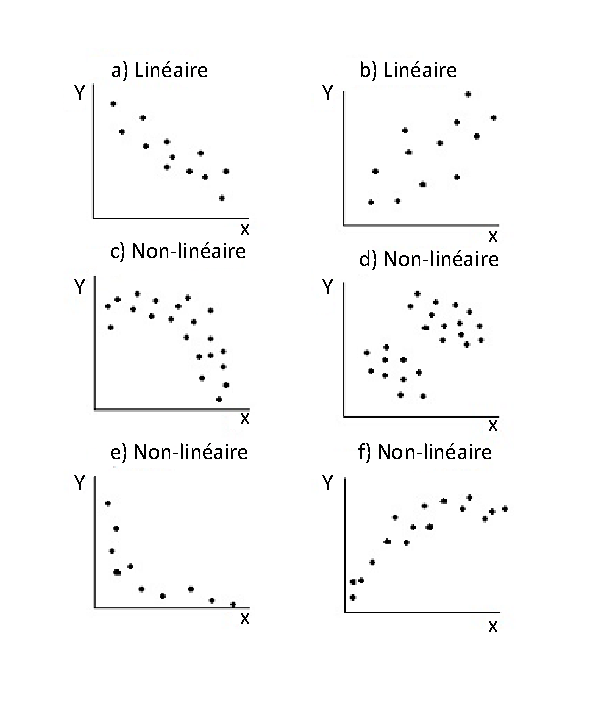
\includegraphics[scale = 1.3]{Chap4-ChoixModeleRLS/Figures/graph_linearite.pdf}
 \caption{Diagramme de dispersion de la variable endogène en fonction de la variable exogène}
 \label{fig:graph_linearite}
\end{figure}

\clearpage

La figure~\ref{fig:graph_linearite_residus} illustre quatre diagrammes de dispersion des résidus en fonction des valeurs prédites. Si le postulat de linéarité est raisonnable, ce graphique devrait montrer un nuage de points centré verticalement en 0. Le nuage de points devrait exhiber une allure complètement aléatoire, c'est-à-dire
qu'il ne devrait exister aucune tendance discernable (par exemple résidus croissants ou décroissants en fonction de $Y_i$, graphique à l'allure quadratique, etc.). Dans cet exemple, seul un diagramme résulte d'une relation linéaire. Les vraies relations desquelles sont issues les données sont indiquées dans le titre des graphiques.

\begin{figure}[htbp]
 \centering
  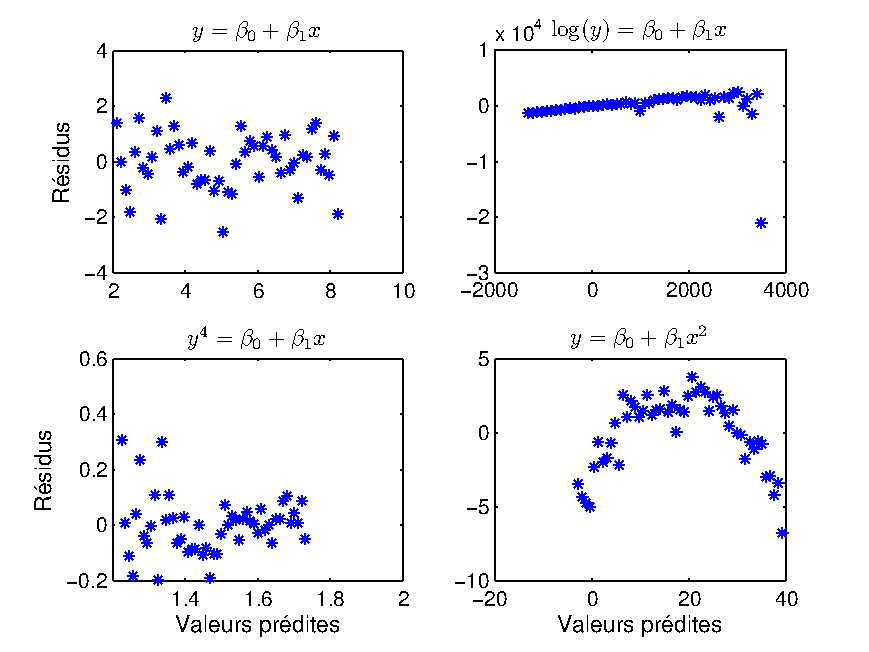
\includegraphics{Chap4-ChoixModeleRLS/Figures/Residus_yhat_Regress_log_ycarre_quadratique.pdf}
 \caption[Exemples de quatre diagrammes de dispersion des résidus en fonction des valeurs prédites.]{Exemples de quatre diagrammes de dispersion des résidus en fonction des valeurs prédites. Dans les quatre cas, le modèle de régression linéaire simple a été ajusté aux données. Le titre de chaque graphique indique le vrai modèle duquel les données sont issues.}
 \label{fig:graph_linearite_residus}
\end{figure}

\clearpage

La figure~\ref{fig:graph_linearite_residus_x} montre quatre diagrammes de dispersion des résidus en fonction de la variable exogène. Comme dans la figure~\ref{fig:graph_linearite_residus}, si le postulat de linéarité est vérifié, ce graphique devrait montrer un nuage de points centré verticalement en 0 et à l'allure aléatoire. À nouveau seul un diagramme est issu d'une relation linéaire. En comparant ces diagrammes en nuages de points avec ceux de la figure~\ref{fig:graph_linearite_residus}, nous constatons que ces deux types de graphiques sont similaires et permettent de tirer les mêmes conclusions.

%\vspace{0.1 in}

\begin{figure}[htbp]
\centering
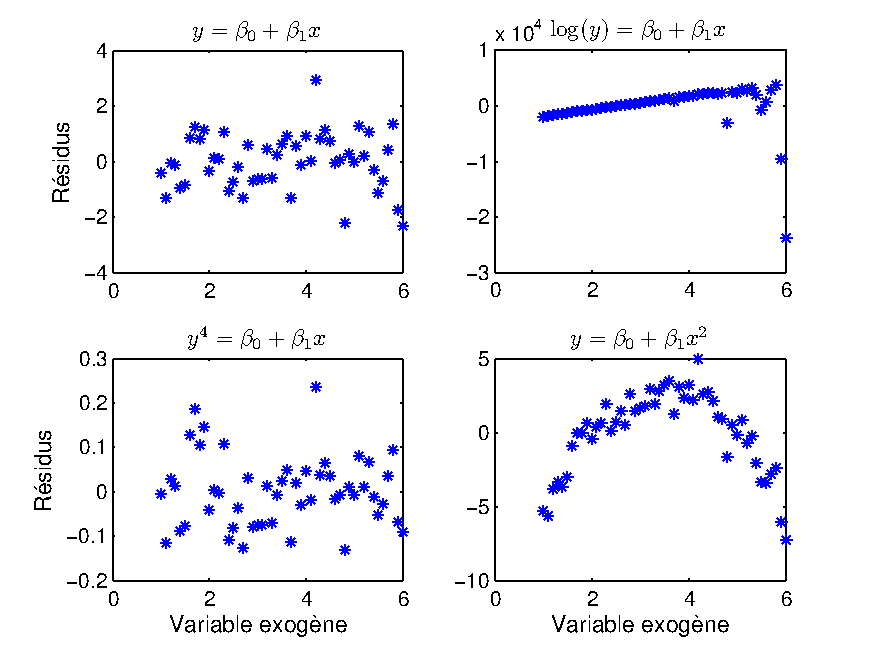
\includegraphics[scale = 0.9]{Chap4-ChoixModeleRLS/Figures/Residus_x_Regress_log_ycarre_quadratique.pdf}
\caption[Exemple de quatre diagrammes de dispersion des résidus en fonction de la variable exogène.]{Exemple de quatre diagrammes de dispersion des résidus en fonction de la variable exogène. Dans les quatre cas, le modèle de régression linéaire simple a été ajusté aux données. Le titre de chaque graphique indique le vrai modèle duquel les données sont issues.}
 \label{fig:graph_linearite_residus_x}
\end{figure}


Il est très important d'examiner les graphiques~\ref{fig:graph_linearite} et \ref{fig:graph_linearite_residus} ou \ref{fig:graph_linearite} et \ref{fig:graph_linearite_residus_x}. Si la relation n'est pas linéaire, la régression linéaire simple ne constitue pas un modèle approprié. Il est alors possible de transformer les données pour obtenir une relation linéaire (voir la \autoref{sec:transfoRLS}). Par exemple, dans le cas d'une relation du type de celles présentées à la figure \ref{fig:graph_linearite} e) et f), on peut tenter un modèle du genre:
 \[1/Y_i = \beta_0 + \beta_1 (1/x_i) + \varepsilon_i
\]
ou
 \[\log(Y_i)= \beta_0 + \beta_1 \log(x_i) + \varepsilon_i.
\]

\begin{remarque}
Les résidus standardisés devraient en général se situer entre -3 et 3, car si le modèle de régression linéaire simple est approprié, ils sont issus d'une distribution normale centrée réduite. On peut vérifier si c'est le cas à l'aide des graphiques utilisés pour tester la linéarité. Si certains résidus possèdent des valeurs plus grandes que 3 en valeur absolue, ceci peut indiquer un manque de normalité, qui sera discuté sous peu, ou la présence de données aberrantes, dont nous reparlerons au \autoref{sec:DonneesInfluentes}.
\end{remarque}


\subsection{Homoscédasticité}
\label{sec:Homoscédasticité}
On a vu que le graphique des résidus standardisés en fonction des valeurs prédites permet de vérifier la linéarité. Le même graphique permet de juger de l'homoscédasticité ($\var[\varepsilon_i]=\sigma^2 \ \ \ 1 \leq i \leq n$). L'hétéroscédasticité signifie que la variance des résidus n'est pas constante. Un graphique pour lequel la variabilité des résidus semble différente pour différentes valeurs des valeurs prédites indique un tel problème. La figure \ref{fig:graphs_homoscedasticite} illustre de façon schématique divers problèmes d'hétéroscédasticité.

\vspace{0.1 in}
\begin{figure}[htbp]
 \centering
  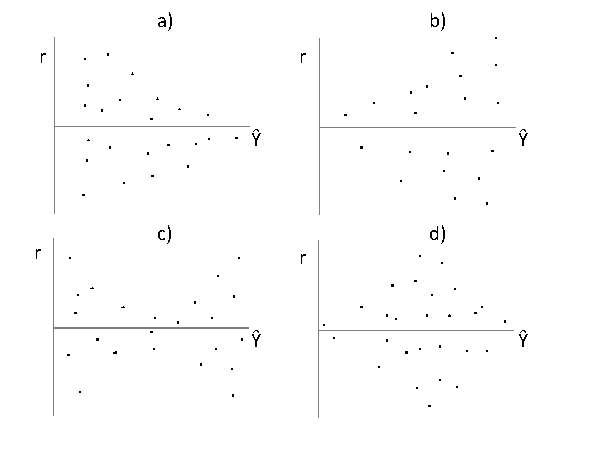
\includegraphics{Chap4-ChoixModeleRLS/Figures/graphs_homoscedasticite}
 \caption{Exemples d'hétéroscédasticité illustrée avec le graphique des résidus standardisés.}
 \label{fig:graphs_homoscedasticite}
\end{figure}

Pour régler le problème d'hétéroscédasticité, on peut également envisager une transformation de la variable endogène.

\newpage
\subsection{Indépendance}
\label{sec:Indépendance}

L'indépendance des observations est plus difficile à tester.

Si les données sont chronologiques, on peut tracer le graphique des résidus en fonction du numéro d'observation. Si aucun patron n'est détecté, le postulat d'indépendance est valable. Sinon, il existe peut-être de l'autocorrélation entre les données (dépendance temporelle). La figure \ref{fig:graphs_autocorrelation} montre un exemple d'autocorrélation positive, et un exemple d'autocorrélation négative. D'autres types de dépendance sont également possibles.


\begin{figure}[h]
\centering
  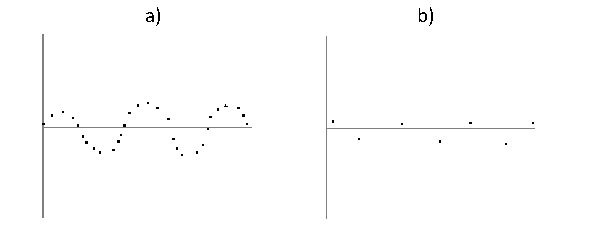
\includegraphics[scale = 1.5]{Chap4-ChoixModeleRLS/Figures/graphs_autocorrelation}
  \caption{Exemple d'autocorrélation positive (a) et négative (b)}
  \label{fig:graphs_autocorrelation}
\end{figure}


Si les données ne sont pas chronologiques, on peut parfois réaliser que $\mathcal{P}_3$ n'est pas valide en analysant la méthode avec laquelle les données ont été collectées. Par exemple, si plusieurs données viennent d'une même unité, il se peut que leurs erreurs soient corrélées.


\subsection{Normalité}
\label{sec:Normalité}


Ce postulat est moins critique que les autres. En effet, même si l'hypothèse de normalité n'est pas vérifiée, $\hat{\beta}_0$, $\hat{\beta}_1$ et $\hat{\sigma}^2$ possèdent un sens dans le cadre du modèle. En revanche, les intervalles de confiance, les tests et les seuils observés sont tous biaisés en l'absence de normalité. Il est possible de vérifier la normalité par des méthodes graphiques (histogramme,  diagramme en boîte (boxplot), droite de Henry) ou par des tests formels (Shapiro-Wilk et Kolmogorov-Smirnov). Dans tous les cas, ces tests sont basés sur les résidus standardisés, car même si ces derniers sont dépendants, ils présentent l'avantage de posséder la même variance.

\subsubsection{L'histogramme}
\label{sec:LHistogramme}

L'histogramme permet de vérifier la symétrie et l'unimodalité. Une distribution normale est unimodale et symétrique, comme illustré à la figure \ref{fig:distresidus}a).

\begin{figure}[htbp]
 \centering
  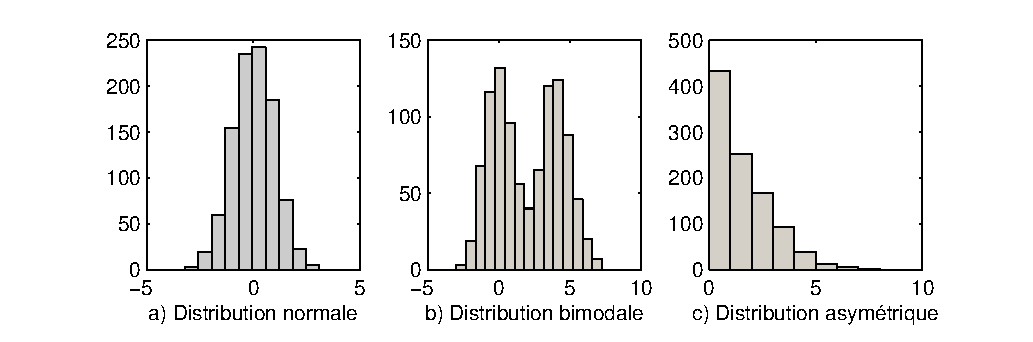
\includegraphics[width=1.00\textwidth]{Chap4-ChoixModeleRLS/Figures/distresidus}
 \caption[Histogramme présentant la distribution des résidus.]{Histogramme présentant la distribution des résidus. Seule la distribution normale (a) est jugée acceptable. Dans les cas b) et c), le modèle apparaît comme n'étant pas adéquat.}
 \label{fig:distresidus}
\end{figure}

\subsubsection{Le diagramme en boîte}
\label{sec:LeDiagrammeÀMoustache}

Le diagramme en boîte, aussi appelé diagramme à moustaches ou \textit{ boxplot} en anglais, permet de vérifier la symétrie, tout comme l'histogramme. Il permet aussi d'identifier la présence de valeurs extrêmes. Une valeur est considérée comme extrême (et indiquée par un symbole particulier) si elle est à l'extérieur des bornes $$\hat q(25\%)-1,5 \times \left\{\hat q(75\%)-\hat q(25\%)\right\} \mbox{   ,    } \hat q(75\%)+1,5 \times \left\{\hat q(75\%)-\hat q(25\%)\right\}$$ où $\hat{q}(\cdot)$ désigne le quantile empirique. Trop de valeurs extrêmes indiquent un problème de normalité, un problème potentiel lors de l'échantillonnage, un problème de linéarité ou alors la présence de deux populations distinctes.

 La figure \ref{fig:boxplot_residus} montre trois diagrammes en boîte des résidus. Le diagramme de gauche est typique d'une distribution normale, celui du centre illustre la présence de valeurs extrêmes indiquées par le symbole $+$, alors que le diagramme de droite reflète une asymétrie des résidus.

\newpage

\begin{figure}[htbp]
 \centering
  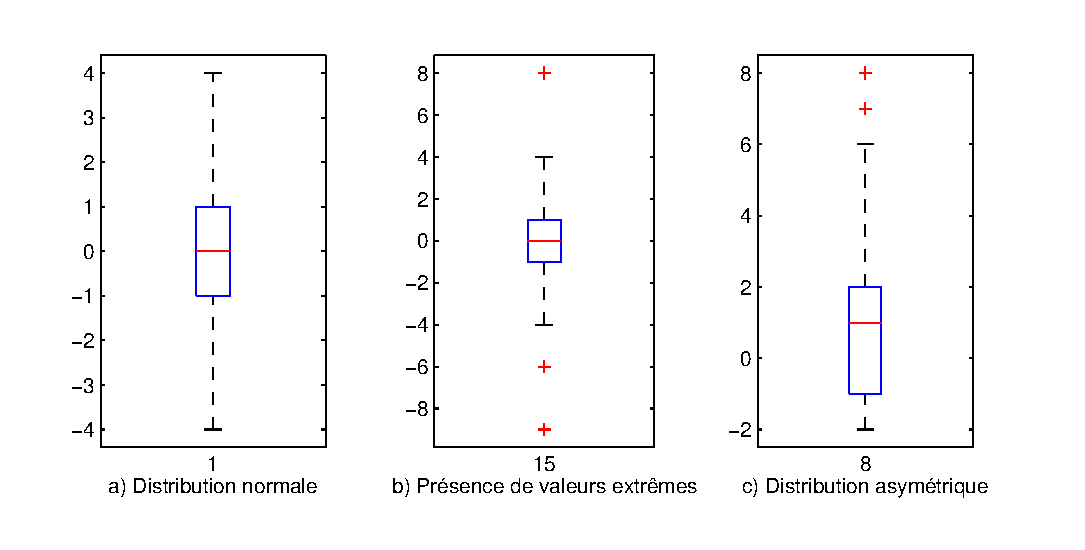
\includegraphics[scale = 0.7]{Chap4-ChoixModeleRLS/Figures/boxplot_residus.eps}
 \caption{Exemple de diagrammes en boîte représentant les résidus.}
 \label{fig:boxplot_residus}
\end{figure}


\subsubsection{Le diagramme quantile-quantile normal}
\label{sec:LaDroiteDeHenry}


L'idée de base ici est que si un échantillon suit une certaine loi, les quantiles empiriques observés dans les données devraient être similaires aux quantiles théoriques de cette loi. Ainsi,  un graphique des quantiles empiriques versus les quantiles théoriques devrait ressembler à une droite de pente 1 passant par l'origine.

On nomme diagramme quantile-quantile normal (\textit{normal QQ-plot}) le nuage de points qui illustre les quantiles empiriques en fonction des quantiles théoriques. Puisqu'on souhaite tester la normalité des résidus, on utilise les $n$ quantiles théoriques de la loi normale centrée réduite, qu'on compare aux quantiles empiriques des résidus standardisés $r_i$.

Un deuxième type de graphique très similaire compare plutôt les statistiques d'ordre théoriques avec les valeurs observées. On le nomme habituellement droite de Henry.\footnote{Le terme droite de Henry est parfois utilisé aussi pour un QQ-plot qui teste la normalité.} Voici concrètement comment le construire:

\begin{enumerate}
 \item On ordonne les résidus standardisés $r_{i}$, qu'on note $r_{(i)}$.
 \item On calcule l'espérance des statistiques d'ordre de la loi normale centrée réduite donnée par $$u_{(i)}=\esp[Z_{(i)}]=\int_{-\infty}^{\infty}zn{n-1 \choose i-1}\Phi^{i-1}(z)\varphi(z)dz$$ où $\varphi(z)=\frac{1}{\sqrt{2\pi}}\exp(-z^2/2)$ et $\Phi(z)=\int_{-\infty}^z\varphi(t)dt$. Lorsque $n$ est grand, il est possible d'utiliser l'approximation suivante $\esp[Z_{(i)}]= \Phi^{-1} \left(\frac{i-3/8}{n-1/4}\right)$.
 \item On trace le graphique de $r_{(i)}$ en fonction de $u_{(i)}$
\end{enumerate}

Si les résidus sont normaux, les points devraient être alignés. Lorsque les points forment une courbe concave ou convexe, la distribution des résidus est non
symétrique. Un graphique en forme de S  indique un aplatissement différent de la
 distribution  normale. La figure \ref{fig:qqplot_residus} montre des exemples de droites de Henry. Le graphique a) illustre le cas d'une distribution normale alors que les deux autres graphiques indiquent respectivement des queues trop lourdes (b) et trop légères (c).
\begin{figure}[htbp]
 \centering
  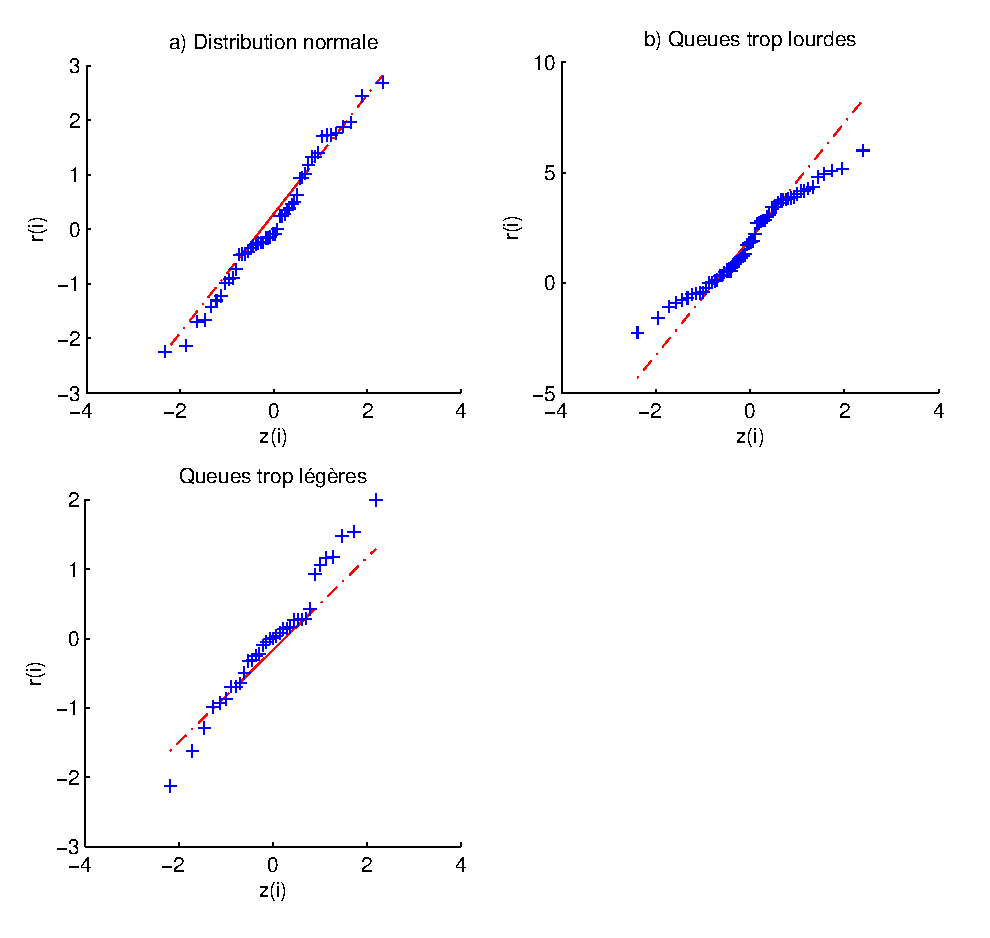
\includegraphics[scale = 0.7]{Chap4-ChoixModeleRLS/Figures/qqplot_residus.eps}
 \caption{Droites de Henry }
 \label{fig:qqplot_residus}
\end{figure}


\vspace{-0.1in}
\subsubsection{Tests formels}

Les graphiques suffisent fréquemment pour confirmer ou infirmer les postulats du modèle. Cependant il n'est pas rare que l'interprétation de certains graphiques soit difficile et puisse paraître ambiguë. Dans ces cas, il existe certains tests d'hypothèses formels permettant de vérifier les postulats. La possibilité de faire un test formel ne signifie toutefois pas qu'il faille négliger les approches graphiques, car ces dernières permettent d'identifier ce qui crée la non-normalité (asymétrie, valeurs extrêmes), ce que les tests formels ne permettent pas de faire.


\newpage
Nous présentons ici deux tests de normalité. Les hypothèses dans les deux cas sont
\begin{align*}
H_0: & \mbox{ Les erreurs sont distribuées selon une loi normale.}\\
H_1: & \mbox{ Le postulat de normalité des erreurs n'est pas vérifié.}
\end{align*}
De grandes valeurs de $p$ indiqueront donc que l'hypothèse de normalité est respectée.

\textbf{Test de Shapiro-Wilk}

La statistique du test de Shapiro-Wilk est la suivante:
\begin{align*}
 W= \frac{\left(\sum_{i=1}^n a_i r_{(i)} \right)^2}{\sum_{i=1}^n (r_i-\overline{r})^2} & \hspace{2cm} \mbox{où} & a_i &= \frac{\overline{Z}^T V^{-1}}{\sqrt{\overline{Z}^T V^{-1}\overline{Z}}}\\
 & &\overline{Z} &= (\esp[Z_{(1)}],...,\esp[Z_{(n)}])
\end{align*}
Ici, $Z_{(i)}$ est la $i^e$ statistique d'ordre d'une loi normale centrée réduite, $V$ est la matrice de variance-covariance des $Z_{(i)}$, et $\overline r=0$.

La statistique $W$ est à peu près équivalente à un coefficient de détermination entre les variables $r_{(i)}$ et $u_{(i)} = \esp(Z_{(i)})$. On peut ainsi faire le lien entre la droite de Henry et la statistique de Shapiro-Wilk. En effet une valeur de $W$ proche de 1 indique un bon alignement des points sur la droite de Henry. L'avantage du test de Shapiro-Wilk est qu'il permet de faire un test formel basé sur la distribution de $W$ sous l'hypothèse nulle que $W=1$. Les logiciels fournissent une $p$-valeur pour ce test.

\textbf{Le test de Kolmogorov-Smirnov}

De façon générale, le test de Kolmogorov-Smirnov permet de tester si un échantillon suit une loi quelconque, de répartition $F$. Ce test est basé sur la distance entre cette loi  sous $H_0$ (notée $F_0$) et l'estimation non paramétrique de $F$, c'est-à-dire la fonction de répartition expérimentale
 \[ F_n (x)=\frac{1}{n} \sum_{i=1}^n \I (x_i \leq x) \ \ \ \ \ \ \ x\in \R.
\]

Lorsque $n \rightarrow \infty$, $ F_n (x) \rightarrow F_0 (x)$. Dans le cadre de la régression, on souhaite tester si l'échantillon suit une loi normale. L'hypothèse nulle du test est donc $H_0: F_0$ est la distribution normale. La statistique du test est:
\begin{eqnarray*}
 D_n = \sup_{x} \left|F_n (x) - F_0 (x) \right|
\end{eqnarray*}

Si l'hypothèse nulle est vraie, alors $D_n$ est proche de 0. Les logiciels fournissent une $p$-valeur pour le test de Kolmogorov-Smirnov. Bien que très utilisé, ce test est peu puissant et on lui préfère le test de Shapiro-Wilk.


\subsection{Exemple}

Les données de la section \ref{exemple-RLS-interpretation} ne sont pas très intéressantes pour vérifier la validité des postulats étant donné que la relation linéaire est presque parfaite. On s'intéressera plutôt ici à la concentration d'ozone dans l'atmosphère.

La pollution de l'air constitue une préoccupation majeure de santé publique. De nombreuses recherches ont démontré l'influence sur la santé de certains composés chimiques tels l'ozone (O$_3$). Certaines catégories de la population, tels les nouveaux-nés, les personnes âgées et les personnes asthmatiques, sont particulièrement sensibles à la pollution. La prévision des pics de concentration des polluants revêt par conséquent une grande importance.

Les lois de la chimie nous informent que cette concentration augmente avec la température. L'association de la surveillance de la qualité de l'air en Bretagne (nommée \texttt{Air Breizh}) mesure depuis plusieurs années la concentration en ozone toutes les 10 minutes ainsi que des données météorologiques comme la température et le vent à certaines heures de la journée.  L'objectif de cet exemple consiste à prédire le maximum journalier de concentration d'ozone en fonction de la température à 12h. Pour cela on se base sur un échantillon de 112 observations mesurées du 1er juin au 30 septembre 2001 par \texttt{Air Breizh}. Pour plus de détails concernant la base de données, le lecteur se référera à  \citet[][Section 1.1.1]{Cor_Mat:07}.
%Les données sont disponibles sur le site web de Pierre-André Cornillon à l'adresse \url{http://www2.agrocampus-ouest.fr/math/livreR/ozone.txt}. Inactif

On choisit comme modèle la régression linéaire simple. La variable endogène est la concentration maximale d'ozone mesurée dans une journée, en $\mu$g/ml (maxO3). La température à 12h (T12) constitue la variable exogène. Le modèle s'exprime donc:
\begin{eqnarray*}
  \max \mbox{O}3 &=& \beta_0 + \beta_1 \mbox{T}12 +\varepsilon.
\end{eqnarray*}
On peut calculer que $\hat{\beta_0} = -27,42$ et que $\hat{\beta_1} = 4,65$.

%Les postulats du modèle comprennent : 1) la linéarité de la relation, 2) l'homoscédasticité, 3) l'indépendance et 4) la normalité des résidus.
%Comme l'objectif est une prévision, le postulat de normalité doit être respecté.

Regardons maintenant la validité des postulats. La figure \ref{fig:ozone_FitPlot1} permet de supposer que la linéarité est respectée. Il en va de même pour le graphique des résidus studentisés (figure \ref{fig:ozone_RStudentByPredicted1}). Ce dernier graphique permet en outre de constater que la variance des résidus est constante. Le postulat d'homoscédasticité est donc lui aussi respecté.


\begin{figure}
  \centering
  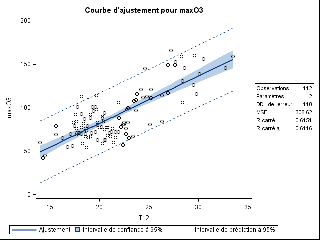
\includegraphics[width=12cm]{Chap4-ChoixModeleRLS/Figures/ozone/FitPlot1.pdf}\\
  \caption[Droite de régression de l'ozone en fonction de la température]{Droite de régression de l'ozone en fonction de la température. Ici, la linéarité ne semble pas causer de problème. Notez que le graphique montre également la droite de régression, l'intervalle de confiance à 95\% (en ombragé bleu) et l'intervalle de prévision (en pointillé).}\label{fig:ozone_FitPlot1}
\end{figure}
\begin{figure}
  \centering
  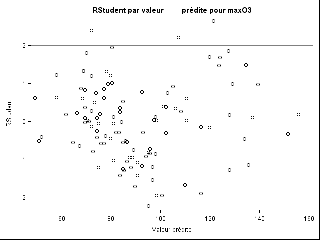
\includegraphics[scale = 2]{Chap4-ChoixModeleRLS/Figures/ozone/RStudentByPredicted1.pdf}\\
  \caption[Graphique des résidus studentisés pour l'exemple de l'ozone]{Graphique des résidus studentisés pour l'exemple de l'ozone. Ce graphique permet de constater que la relation est linéaire et que la variance des résidus est constante.}\label{fig:ozone_RStudentByPredicted1}
\end{figure}

\clearpage

Puisque les données sur l'ozone et la température sont collectées à différents moments, il s'agit d'une série temporelle et il y a un potentiel d'autocorrélation. Le graphique des observations en fonction du numéro d'observation (figure \ref{fig:ozone_independance}) permet en effet de douter de l'indépendance des observations. Ce type de problème est fréquent lorsque l'on travaille avec des données temporelles. Il faudrait dans ce cas faire des tests formels d'autocorrélation. Toutefois, puisque ces tests ne font pas l'objet de ce cours et que les patrons observés sont tout de même vagues, on considérera en pratique que le postulat d'indépendance est respecté.


\begin{figure}[h!]
  \centering
  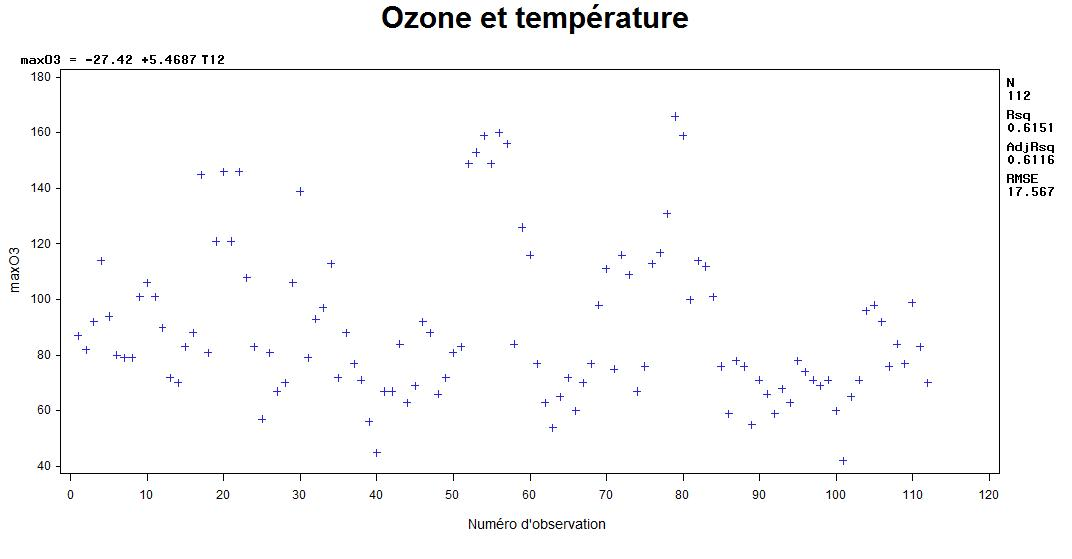
\includegraphics[width=15cm]{Chap4-ChoixModeleRLS/Figures/ozone/independance.jpg}\\
  \caption{Vérification de l'indépendance des observations. On observe quelques vagues patrons qui pourraient signifier qu'il y a autocorrélation.}\label{fig:ozone_independance}
\end{figure}


En ce qui concerne le postulat de normalité, les méthodes graphiques suggèrent toutes que les résidus sont normaux (voir les figures \ref{fig:ozone_ResidualHistogram1}, \ref{fig:ozone_ResidualBoxPlot1} et \ref{fig:ozone_QQPlot1}). Les tests formels confirment le respect du postulat de normalité (tableau \ref{tab:ozone_test_normalite}). La statistique de Shapiro-Wilk est de 0,99. Cette statistique peut être interprétée comme étant le $R^2$ de la droite de Henry. La statistique de Shapiro-Wilk et la figure \ref{fig:ozone_QQPlot1} sont donc cohérentes. L'hypothèse nulle du test de Shapiro-Wilk est que les résidus sont normaux. Avec une $p$-valeur de 0,79, on ne peut pas rejeter cette hypothèse. Quant au test de Kolmogorov-Smirnov, dont l'hypothèse nulle est aussi la normalité des résidus, sa $p$-valeur est supérieure à 0,15. Les deux tests aboutissent donc à la même conclusion: les résidus suivent une distribution normale.

Toutes les hypothèses de la régression linéaire simple sont donc satisfaites pour ce jeu de données.

\newpage

\begin{figure}
\centering
\begin{minipage}{.45\textwidth}
  \centering
  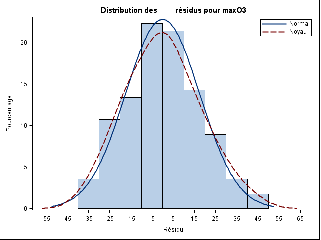
\includegraphics[scale = 1.3]{Chap4-ChoixModeleRLS/Figures/ozone/ResidualHistogram1.pdf}\\
  \captionof{figure}{Histogramme des résidus. La forme de l'histogramme est typique d'une distribution normale.}
  \label{fig:ozone_ResidualHistogram1}
\end{minipage}%
\hspace{1 cm}
\begin{minipage}{.45\textwidth}
  \centering
  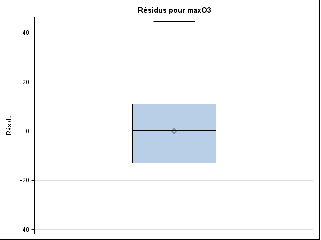
\includegraphics[scale = 1.3]{Chap4-ChoixModeleRLS/Figures/ozone/ResidualBoxPlot1.pdf}\\
  \captionof{figure}{Diagramme en boîte des résidus. Les résidus sont à peu près symétriques et on n'observe aucune valeur extrême.}
  \label{fig:ozone_ResidualBoxPlot1}
\end{minipage}
\end{figure}


\begin{figure}
\centering
  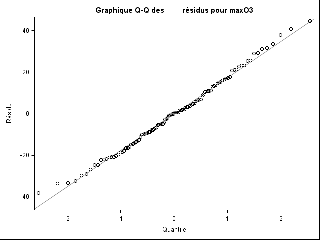
\includegraphics[scale = 1.3]{Chap4-ChoixModeleRLS/Figures/ozone/QQPlot1.pdf}\\
  \caption[Droite de Henry]{Droite de Henry. Les points sont très bien alignés sur la droite; la distribution des résidus semble normale.}
  \label{fig:ozone_QQPlot1}
\end{figure}

\begin{figure}
  \centering
  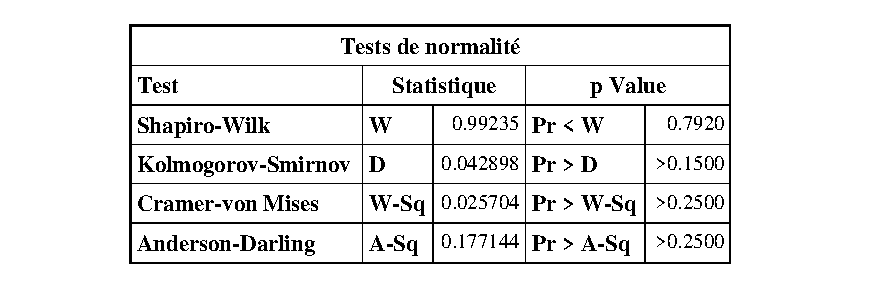
\includegraphics[scale = 0.8]{Chap4-ChoixModeleRLS/Figures/ozone/test_normalite.pdf}\\
  \caption{Résultat des tests de normalité.}
\label{tab:ozone_test_normalite}
\end{figure}

\clearpage

\section{Transformation des données}
\label{sec:transfoRLS}

Si les postulats de la régression ne sont pas respectés, et donc que le modèle \\$y_i~=~\beta_0 ~+~ \beta_1 ~x_i ~+ ~\varepsilon_i$ ne colle pas à la réalité, on peut effectuer une transformation des variables qui permettra d'utiliser le modèle de régression linéaire.  Il existe en effet souvent une fonction $g(\cdot)$ qui transforme une des variables de façon à régler un problème de linéarité, d'hétéroscédasticité ou de normalité. On propose ici trois méthodes pour trouver $g(\cdot)$.



\subsection{La technique de Mosteller et Tukey}
\label{sec:LaTechniqueDeMostellerEtTukey}


La technique de Mosteller et Tukey est une méthode graphique généralement utilisée pour régler un problème de linéarité, mais qui peut aussi être utile dans le cas d'un problème de normalité. On trace simplement le graphique de la variable endogène en fonction de la variable exogène et on observe la forme du nuage de points. %trouver une fonction $g(\cdot)$ appropriée à l'aide des diagrammes de dispersion des couples $[x_i; g(Y_i)]$ pour plusieurs choix de $g(\cdot)$, jusqu'à obtention d'un graphique d'apparence le plus linéaire possible.
La \autoref{fig:Mosteller_Tukey} montre quel type de transformation est appropriée à chaque forme de nuage de points.

\begin{figure}[htb]
 \centering
  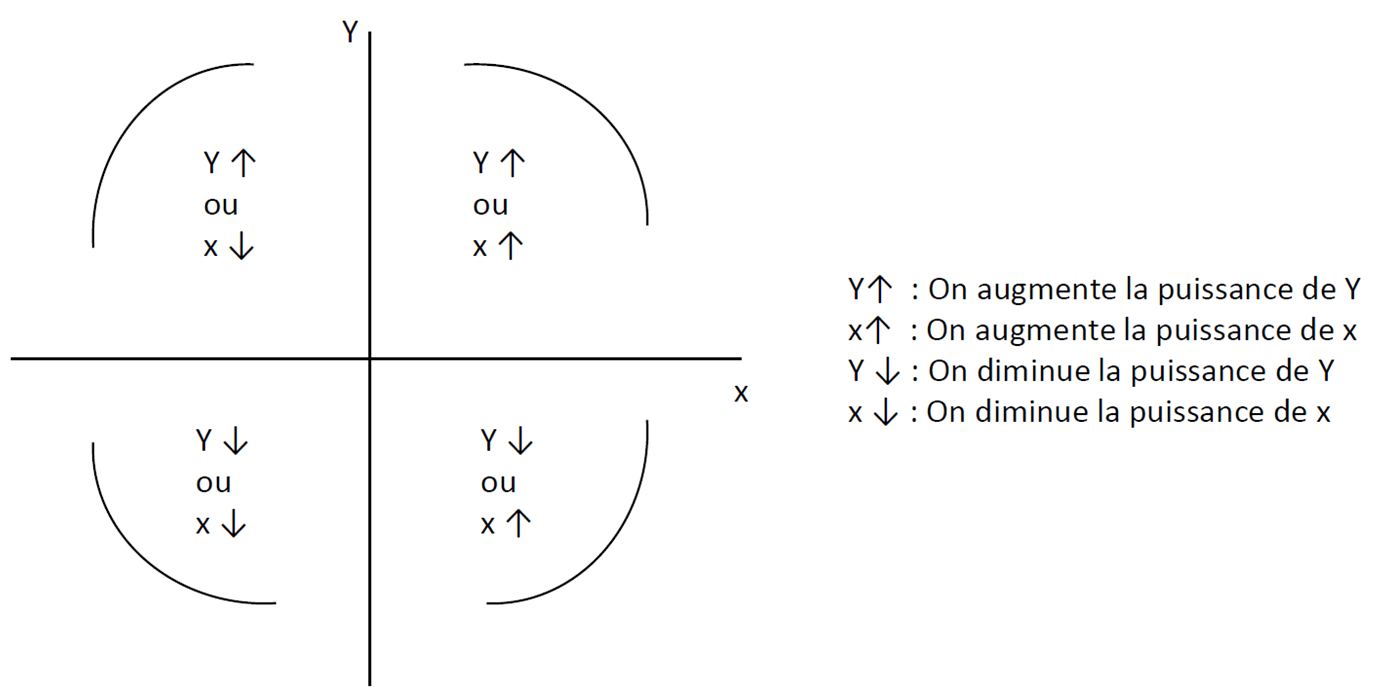
\includegraphics[scale = 0.6]{Chap4-ChoixModeleRLS/Figures/Mosteller_Tukey_2}
 \caption{Transformation des variables avec la technique de Mosteller-Tukey}
 \label{fig:Mosteller_Tukey}
\end{figure}

En pratique, on peut tester plusieurs transformations possibles de la variable endogène et/ou de la variable exogène, telles que suggérées par la méthode. On choisira le modèle pour lequel les hypothèses de la régression linéaire simple semblent le plus valides.

\begin{remarque}
Il vaut mieux si possible appliquer la transformation à la variable exogène plutôt qu'à la variable endogène. La prévision à l'aide du modèle et l'interprétation des intervalles de confiance et de prévision seront plus faciles. Voir section \ref{subsection:previsiontrans}.
\end{remarque}

\subsection{La technique de Box-Cox}
\label{sec:LaTechniqueDeBoxCox}


L'idée de Georges Box et David Cox, publiée en 1964, consiste à généraliser le modèle de régression en introduisant un paramètre supplémentaire $\lambda$ dans le modèle. Plus précisément, on considère le modèle
\begin{eqnarray}
 g(Y_i,\lambda)=\beta_0 + \beta_1 x_i + \varepsilon_i
 \label{eq:reg_box_cox}
\end{eqnarray}
où
\begin{equation}\label{eq:gboxcox}
g(y;\lambda)=\left\{\begin{array}{ll}{y^\lambda-1\over\lambda}, & \lambda\neq0\\
\log(y), & \lambda=0.\end{array}\right.
\end{equation}
et $\lambda$ est un paramètre inconnu à estimer à partir des données.


On suppose la normalité des termes d'erreurs\footnote{La technique peut être contestée du fait de cette hypothèse} et on maximise la vraisemblance par rapport à $\beta_0 , \beta_1, \sigma^2$ et $\lambda$.
Pour cela on pose $W_i(\lambda)=\beta_0+\beta_1 x_i+\varepsilon_i$. Comme on a supposé la normalité des termes d'erreur, on a que $W_i\sim\N(\beta_0+\beta_1 x_i,\sigma^2)$. La vraisemblance s'exprime alors comme
\begin{eqnarray*}
L(\beta_0,\beta_1,\sigma,\lambda)=\prod_{i=1}^n f(W_i)=\prod_{i=1}^n \left(\frac{1}{\sqrt{2\pi\sigma^2}}\right)\exp\left[-\frac{1}{2}\left\{\frac{W_i-(\beta_0+\beta_1 x_i)}{\sigma}\right\}^2\right]J(\lambda),
\end{eqnarray*}
où $J(\lambda)$ note le jacobien de la transformation.

Le problème qui se pose à ce point est que l'on ne peut résoudre $$\frac{\partial L}{\partial \beta_0}=\frac{\partial L}{\partial \beta_1}=\frac{\partial L}{\partial \sigma^2}=\frac{\partial L}{\partial \lambda}=0$$ explicitement. La plupart des logiciels ont des routines pour estimer $\lambda$ numériquement et donnent également un intervalle de confiance pour la valeur de $\lambda$.

Une fois qu'on a estimé $\lambda$, l'\autoref{eq:gboxcox} indique la transformation à utiliser. En pratique, on effectue simplement la régression de $y^{\hat{\lambda}}$ en fonction de $x$.

Si $\lambda = 0$, alors on utilise $\log(Y)$. En effet, $\displaystyle\lim_{\lambda\rightarrow 0}\frac{y^\lambda-1}{\lambda}=\displaystyle\lim_{\lambda\rightarrow 0}\frac{y^\lambda\log(y)}{1}=\log(y).$ Si l'intervalle de confiance de $\lambda$ contient $0$ une transformation logarithmique peut donc être appropriée.

\begin{remarque}
On doit aussi considérer l'interprétation du modèle dans le choix des transformations. Ainsi, une variable à la puissance $1,8765$ est souvent plus difficile à concevoir et à interpréter qu'une variable à la puissance 2. On préférera donc généralement arrondir les puissances.
\end{remarque}

\subsection{Technique de stabilisation de la variance}
\label{sec:Approx_var}

Cette méthode est utilisée en cas de problème d'hétéroscédasticité. Dans ce cas, il y a un lien entre la variation des résidus et les valeurs ajustées. On peut donc dire que la variance des résidus est une fonction de l'espérance de la valeur de $Y$. L'idée est de choisir une transformation $g()$ de sorte que $g(y)$ ait une variance constante.

Le choix des transformations possibles pour stabiliser la variance se base sur la formule approximative pour la variance d'une variable transformée $g(Y)$. Le développement de Taylor du premier ordre conduit à
\begin{eqnarray*}
g(Y)& = & g(\esp[Y]+\{Y-\esp[Y]\}) \\
& \approx  & g(\esp[Y])+g'(\esp[Y])(Y-\esp[Y]).
\end{eqnarray*}
La variance peut donc être approchée par
\begin{eqnarray}
\var[g(Y)]\approx \left\{g'(\esp[Y])\right\}^2\var[Y].
 \end{eqnarray}
 Soit par exemple $Y$ une variable aléatoire telle que son écart-type en fonction de l'espérance est $\sigma(\mu)=\mu^{1/2}$. La substitution dans la formule aproximative pour la variance nous montre que  $\var[g(Y)]\approx \{g'(\mu)\}^2\sigma^2=\{g'(\mu)\}^2\mu.$ La transformation $g(\cdot)$ telle que la variance de $g(Y)$ soit constante doit donc vérifier $g'(\mu)$ proportionnelle à $1/\sqrt{\mu}$, c'est-à-dire $g(Y)=\sqrt Y$ à une constante près.

Lorsque $Y$ prend des valeurs positives, les transformations les plus utiles sont résumées dans le tableau \ref{tab:TransformationHeteroscedasticite}.

{\small
\begin{table}[htbp]
 \centering
 \caption{Transformations envisageables pour régler l'hétéroscédasticité}
  \renewcommand{\arraystretch}{1.6}
  \begin{tabular}{cc}
   \hline
   Transformation typique & Situation \\
   \hline
   $\sqrt{Y}$  & $\var[\varepsilon_i] \propto \esp[Y_i]$ \\
    & (données de type Poisson) \\ \hline
   $\log (Y)$ & $\var[\varepsilon_i] \propto (\esp[Y_i])^2$  \\
   &  (efficace si $Y$ possède une très grande étendue)\\ \hline
   $1/Y$  & $\var[\varepsilon_i] \propto (\esp[Y_i])^4$\\ \hline
   $\arcsin(\sqrt{Y})$ & $Y\in [0,1]$ et $\var[\varepsilon_i] \propto \esp[Y_i] (1-\esp[Y_i])$\\
   & ($Y$ suit une loi Bernoulli)\\
  \end{tabular}
 \label{tab:TransformationHeteroscedasticite}
\end{table}
}



\subsection{Prévision sous transformation}
\label{subsection:previsiontrans}

Il faut être prudent lorsqu'on applique une transformation à la variable endogène. En effet les prévisions sont alors obtenues en termes de la variable endogène transformée. Or, en général on a que,
$$ \esp[g(Y)]\neq g(\esp[Y]).$$ Il est donc incorrect de simplement appliquer la transformation inverse afin d'obtenir une prévision en termes de la variable aléatoire endogène $Y$ de base (non transformée).

La détermination d'un intervalle de confiance est par contre directe, en utilisant le fait que lorsque $g(\cdot)$ est une fonction monotone, on a que
$$\P\{a\leq g(Y)\leq b\}=\P\{g^{-1}(a)\leq Y\leq g^{-1}(b)\},$$ où $g^{-1}$ désigne la transformation inverse.

%\textcolor{red}{Ajouter quelque chose sur la transformation?}

\begin{exemple}
Soit le modèle de régression linéaire simple suivant :
$$\sqrt{Y}=Y_i^*=\beta_0+\beta_1 x_i+\varepsilon_i.$$ Un intervalle de confiance à 90 \% pour $g(Y)$ lorsque $x=x_0$ est donné par $(0,2;2,4)$. On désire trouver un intervalle de prévision à 90 \% pour $Y$ lorsque $x=x_0$. \\
On a que $Y^*=\sqrt{Y}\Leftrightarrow Y=(Y^{*})^2$.\\
L'intervalle de prévision en termes de la variable endogène de base $Y$ sera donc
$$((0,2)^2;(2,4)^2)=(0,04;5,76).$$
%On ne peut toutefois pas obtenir aisément de prévision pour $Y_i$.
\end{exemple}


